\chapter{Event generation and simulation}
\label{sec:MC}

Monte Carlo (MC) event generators bridge the gap between the mathematical description of particle collisions and the complex, experimentally observable final state. 
The term Monte Carlo refers to the stochastic nature of the underlying physics,
in analogy with the gambling district of Monaco.
This chapter outlines the working principles of event generators.
For a detailed explanation one may refer to ref.~\cite{Buckley_2011}.
The last section of this chapter lists the data and MC samples 
that are used for the cross section analysis presented in chapter~\ref{ch:regions}.

\section{Monte Carlo event generators}

Event generators simulate collision events in sequential steps under
the assumption that the individual steps are universal and can be factorized.
The hard scattering interaction is evaluated at the matrix element level, followed by the parton shower and the non-perturbative hadronization into observable hadrons. 
Secondary soft interactions, pileup and the decays of unstable particles complete the generation chain. The event is passed to a full detector simulation. The result is a simulated event that can be directly compared to real collision data.


\subsection{Hard scattering}

The production of heavy particles or highly energetic jets at the LHC
involves the transfer of large momenta. The QCD particles can be 
assumed to be asymptotically free at these energies and the interaction
can be treated perturbatively. 
Features of the process can be computed with Feynman diagrams up
to a fixed order in perturbation theory, as outlined in section~\ref{sec:xsec_definition}.
The momentum of the ingoing particles is sampled from the PDFs,
and the matrix element is then evaluated for the momentum configuration.
The choice which PDF set is used may differ between event generators.
The PDFs are constrained using measurements from many different
physics processes including deep-inelastic scattering, Drell-Yan processes, or
inclusive jet production.
The color-carrying partons produced in the hard scattering
initiate the next simulation step, parton showering.

\subsection{Parton shower}

The matrix element discussed in the previous section simulates the hard process and
describes the momenta of outgoing jets well.
However, no fixed order calculation is sufficient to give a complete picture of the
process, such as the substructure of jets.

Instead, the effect of higher orders is approximated through
a \textit{parton shower} (PS) algorithm.
Partons from the hard matrix element can radiate gluons.
Gluons, carrying color charge themselves, give rise to further
gluon radiation and parton multiplication.
The purpose of the PS is to simulate an evolution in momentum transfer
from the high scales associated with the hard process to the low scales, of order 1 \GeV.
This scale is associated with confinement of partons into hadrons
and perturbation theory is no longer applicable.

The PS is assumed to be independent of the hard process.
It can be illustrated with the example
of $q\bar{q}$ production with an additional gluon from electron positron annihilation
$e^- e^+ \rightarrow q\bar{q}g$.
The cross section can be approximated as~\cite{Buckley_2011}
\begin{equation}
    \frac{\text{d}\sigma_{q\bar{q}g}}{\text{d cos}\vartheta \text{ d}z} \approx
    \sigma_{q\bar{q}}C_F \frac{\alpha_S}{2\pi}\frac{2}{\text{sin}^2\vartheta} \frac{1+(1-z)^2}{z},
    \label{eq:threepartonxsec}
\end{equation}
where the three parton phase space was parametrized by the opening angle
between the quark and the gluon $\vartheta$, and the energy fraction of the gluon $z$.
The color factor $C_F = \frac{N_C^2 - 1}{2N_C}$ can be interpreted as the squared color charge of the quark with $N_C = 3$, the number of colors.

Equation~\eqref{eq:threepartonxsec} shows that the cross section for 
$q\bar{q}g$ production is proportional to that of
$q\bar{q}$. The remaining expression can be
interpreted as the probability for gluon emission, differential in the
kinematics of the gluon.

The expression in equation~\eqref{eq:threepartonxsec} can be transformed to~\cite{Buckley_2011}
\begin{equation}
    \text{d}\sigma \approx \sigma_0 \sum_{\text{partons},i} 
    \frac{\alpha_S}{2\pi}\frac{\text{d}\vartheta^2}{\vartheta^2}\text{d}z P_{ab}(z,\varphi)d\varphi
    \label{eq:splitting}
\end{equation}
by introducing the splitting functions 
$P_{ab}(z,\varphi)$.
They are a set of universal, but flavor-dependent functions.
Spin dependence is introduced through the azimuthal angle $\varphi$
of $j$ with respect to parton $i$.
The indices in $P_{ab}$ are chosen such that
for the process $a\rightarrow bc$, parton $c$ is fixed by $a$ and $b$.

Equation~\eqref{eq:splitting} is a completely general expression for any hard
process with a collinear splitting.
The splitting of a hard process is treated as the new hard process.
By iterating this step, the parton shower simulates a succession of
emissions from the incoming and outgoing partons.


The differential cross section diverges at the edges of the phase space
when the gluon becomes collinear with the quark
($\vartheta \rightarrow 0$), or with the anti-quark ($\vartheta \rightarrow \pi$),
or when the gluon energy goes to zero ($z \rightarrow 0$).

A cutoff scale $Q_0$ is introduced, typically the minimum relative 
transverse momentum between the partons.
The partons can be resolved, only if $Q_0$ is exceeded.
Thus, resolving the soft and collinear divergences,
resulting in a finite probability of  resolvable emissions.

\subsection{Hadronization}

Once the radiated partons reach the hadronization scale, the shower is terminated.
Phenomenological models have to be introduced to model the formation of observable color-neutral hadrons, as
perturbative QCD calculations are no longer applicable.
The two main models employed in MC generators are illustrated in Figure~\ref{fig:cluster_string}.
\begin{figure}
    \centering
    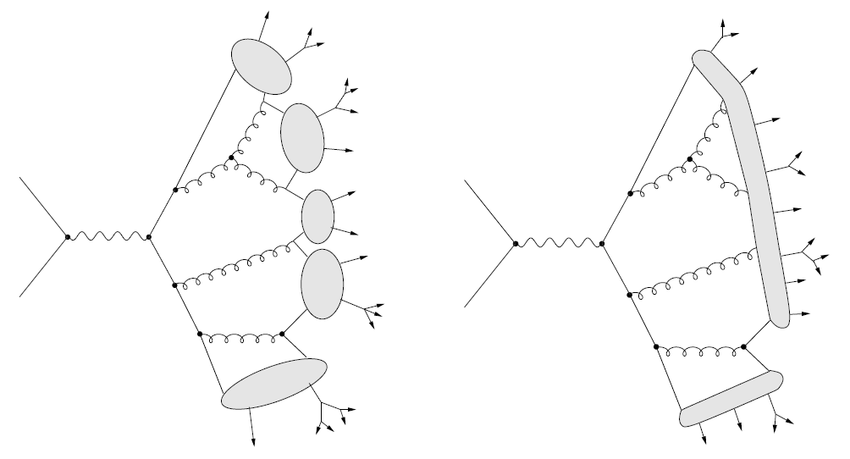
\includegraphics[width=0.5\linewidth]{figures/other/cluster_string_hadronization.png}
    \caption{Illustration of cluster (left) and string (right) hadronization models~\cite{webber1999fragmentationhadronization}.}
    \label{fig:cluster_string}
\end{figure}

In the Lund string model~\cite{ANDERSSON198331}, the color field between a $q\bar{q}$ pair is represented by a relativistic string and gluons give rise to ‘kinks’ on the string.
As the pair moves apart, the string stretches and the potential energy stored in it increases.
When sufficient energy has accumulated the string breaks, producing a new $q\bar{q}$ pair.
The process repeats until the invariant mass of the remaining string segments is too small for further breaking to be kinematically possible.

The cluster model~\cite{WEBBER1984492} is based on the color preconfinement property~\cite{AMATI197987} which
states the tendency of partons
generated in the branching process to be arranged in color-singlet clusters.
These clusters are the basic units out of which hadrons arise non-perturbatively.
Since local clusters are considered, this approach
is independent of the hard process and the center-of-mass energy.


\subsection{Hadron decay}

The hadrons produced in the previous stage can be unstable and decay
before they reach the detector. Therefore, the decay into particles that
can be considered stable on collider timescales is simulated in the last step.

The Particle Data Group (PDG) provides an extensive collection of particle
properties in its Review of Particle Physics~\cite{PhysRevD.110.030001}.
The provided information may not be sufficient,
when considering excited states and hadrons with heavy quarks.
Thus, a choice has to made which hadrons are included in the simulation.
Closely related is the choice of which decay modes are included and how they are simulated.

The specific settings are generator dependent and
closely connected with the tuning of hadronization parameters.


\subsection{Underlying event and pileup}

Beyond the hard process, the incoming hadrons carry additional partons that can undergo softer secondary interactions, collectively referred to as the underlying event. 
Furthermore, multiple proton-proton collisions occurring within the same bunch crossing contribute as pileup.
Both effects are incorporated into the simulation through phenomenological models tuned to experimental data.

\subsection{Detector simulation}

After the generation and showering of simulated events, the final-state stable particles are propagated through a full simulation of the ATLAS detector. 
This  \textsc{Geant}4 software package~\cite{Agostinelli:2002hh} is used to 
simulate the response of the ATLAS detector, 
converting particle-level truth information into realistic detector-level signals.
The full event reconstruction chain, described in Chapter~\ref{chap:ObjectReco}, is then applied using the same algorithms as for real collision data. This yields simulated events that additionally contain generator and truth-matching information not present in recorded data. The procedure is essential for estimating signal acceptance and efficiency, modeling backgrounds, and validating theoretical predictions against measurement.

Some modeling uncertainties are estimated with the the fast-simulation package
\textsc{AtlFast-II}~\cite{SOFT-2010-01}, since a
full simulation of the detector response is computationally expensive.
The package parametrizes hadronic
showers in the electromagnetic and hadronic calorimeter to speed up the simulation.

\subsection{Particle and detector level}

After the full simulation chain, two distinct levels of information are available for analysis. The \textit{detector level} refers to events that have passed through a detailed simulation of the detector response. Ideally, this would be indistinguishable from real collision data. The \textit{particle level} refers to the truth information available before the detector simulation.
It consists of stable hadrons and leptons emerging from the MC generation chain. It is independent of the specifics of any particular experiment.
Physics objects such as jets can be reconstructed directly from particle-level inputs.
The availability of both levels is crucial for data analyses. It allows the detector response to be corrected for in order to reveal the underlying physics.

\section{Data and simulation samples}

This section lists all data samples analyzed in the measurement.
It also introduces the samples that were used to simulate signal and background events.

\subsection{Data samples}

The analyzed data set was taken by the ATLAS experiment between 2015 and 2018.
Proton proton collisions at $\sqrt{s}=13\TeV$ corresponding to an integrated luminosity
of $140.1\pm1.2 \text{ fb}^{-1}$ are analyzed.
The partial integrated luminosities for each year of operation are reported in Table~\ref{tab:Data:Lumi}.
A single-electron or single-muon trigger is employed in the event selection~\cite{TRIG-2018-05, TRIG-2018-01}.
A matching between the object firing the trigger and the offline reconstructed object is required.
\begin{table}[htbp]
    \centering
    \caption{Integrated luminosity for each year of data taking.}%
    \begin{tabular}{ c c }
      \hspace{1pt}\\
      \toprule
      \textbf{Year} & \textbf{Int. Lumi. [fb$^{-1}$]} \\
      \midrule
      2015  & $3.2$ \\
      2016  & $33.4$ \\
      2017  & $44.6$ \\
      2018  & $58.8$ \\
      \midrule
      Run 2 & 140.1\\
      \bottomrule
  \end{tabular}
  \label{tab:Data:Lumi}
\end{table}

\subsection{Monte Carlo simulated samples}%
\label{sec:datamc:mc}

Contributions to the \WbWb final state from SM processes are modeled using Monte Carlo (MC) simulated samples~\cite{SOFT-2010-01}. An overview on all simulated processes is given in 
Table~\ref{tab:physics_samples}.
Three sample categories are distinguished.

The nominal signal is defined as the sum of \ttbar and \tW samples in the DR description.
Both contributions are simulated with the same combination of hard-process generator and parton shower.
The top mass was set to $m_t = 172.5\GeV$.
All \ttbar and \tW events with at least one lepton in the final state are taken into account in the signal region. That includes dilepton events that pass the selection due to out-of-acceptance effect.

Alternative signal samples are used for the comparison to the data.
The nominal \ttbar signal sample is combined with a  DS scheme \tW sample to 
investigate interference effects, as well as to models with alternative PS.
Another key purpose of the alternative samples is the evaluation of modeling systematic uncertainties (see Sec.~\ref{sec:theory_modeling}).

Events from processes other than $WbWb$ may enter the signal region 
by mimicking the the characteristics of the signal process.
Their contribution is mostly estimated from background samples.
They will be evaluated on detector level and removed in the extraction of the
cross sections (see Sec.~\ref{sec:unfolding}).
The dominating background process are \Wjets events. 
Other backgrounds are grouped in the categories ``\OtherV`` and ``\OtherT''.
The columns of Table~\ref{tab:physics_samples} will be briefly explained in the following.

The particular physics process that is modeled in the sample and the corresponding
legend entries in the plots presented in Chapter~\ref{ch:WbWb} are listed in the first two columns.

The matrix element of the hard interaction is modeled using the
\POWHEGBOX[v2]~\cite{Frixione:2007nw,Nason:2004rx,Frixione:2007vw,Alioli:2010xd}
generator. It provides matrix elements at NLO in \alphas, and uses the
\NNPDF[3.0nlo]~\cite{Ball:2014uwa} PDF set as input.
The functional form of the scales $\mu_R$ and $\mu_F$ was
set to the default scale \(\sqrt{\mtop^{2} + p_\mathrm{T\ top}^2}\) in the nominal \ttbar sample.
For the \tW sample the dynamic scale \( \HT / 2 \)~\cite{ATL-PHYS-PUB-2021-042} was selected with
the either the DR (nominal) or DS (alternative) scheme to handle the interference with \ttbar production.
The production of \(V+\)jets was simulated with the \SHERPA[2.2]~\cite{Bothmann:2019yzt}
generator and the \NNPDF[3.0nnlo] PDF set~\cite{Ball:2014uwa,Carrazza:2015aoa}.
%madgraph
The \MGNLO[2.3.3]~\cite{Alwall:2014hca}
generator was used to model the production of \ttV events.
It provides matrix elements at NLO in  \alphas
and uses the \NNPDF[3.0nlo]~\cite{Ball:2014uwa} PDF.
%The functional form of the renormalization and
%factorization scales was set to the default of
%\(0.5 \times \sum_i \sqrt{m^2_i+p^2_{\mathrm{T},i}}\),
%where the sum runs over all the particles
%generated in the matrix element calculation. 
Top quarks were decayed at LO using \MADSPIN~\cite{Frixione:2007zp,Artoisenet:2012st} to
preserve spin correlations. 

Several models were used to simulate PS and hadronization, depending on the sample.
The events from the nominal samples were interfaced with
\PYTHIA[8.230]~\cite{Sjostrand:2014zea}, using the A14 set of tuned
parameters~\cite{ATL-PHYS-PUB-2014-021} and the \NNPDF[2.3lo]
set of PDFs~\cite{Ball:2012cx}.
The decays of bottom and charm hadrons were simulated using the
\EVTGEN[1.6.0] program~\cite{Lange:2001uf}.
The \SHERPA samples employ the default \SHERPA parton showering algorithm~\cite{Schumann:2007mg} instead
with a dedicated set of tuned parameters developed by the
\SHERPA authors and the Hessian \NNPDF[3.0nnlo] PDF set.
Alternative signal samples were obtained by interfacing the same
\POWHEGBOX[v2] set-up to \HERWIG[7.1.3]~\cite{Bellm:2015jjp,Bahr:2008pv}.
%which includes an angular-ordered parton-shower model with a different hadronization model.
This sample was generated using the \HERWIG[7.1]
default set of tuned parameters and the \MMHT[lo] PDF set~\cite{Harland-Lang:2014zoa}.

The samples are normalized to the expected cross sections at $\sqrt{s}=13\TeV$,
the center of mass energy of Run 2. The values are extracted from Refs.~\cite{
Glasman:2765035, Campbell2021, Ball_2022, Kidonakis:2021vob, PhysRevD.81.054028}
and are provided in the last column.
The \ttbar samples are normalized to the cross-section prediction at
NNLO in QCD including the resummation of
next-to-next-to-leading logarithmic (NNLL) soft-gluon terms calculated using
\TOPpp[2.0]~\cite{Beneke:2011mq,Cacciari:2011hy,Baernreuther:2012ws,Czakon:2012zr,Czakon:2012pz,Czakon:2013goa,Czakon:2011xx}.
% tW xsec
For the \tW sample, the inclusive cross-section was corrected to the theory prediction
calculated at NLO in QCD with NNLL soft-gluon
corrections~\cite{Kidonakis:2021vob}.
The \(V\)+jets samples were normalized to a NNLO prediction~\cite{Anastasiou:2003ds}.



\begin{sidewaystable}
    \centering
    \caption{Summary of Signal and Background Samples}
    \label{tab:physics_samples}
    \scriptsize
    \begin{tabularx}{\textheight}{c c c c c c c}
        \toprule
        \multicolumn{7}{c}{\textbf{Nominal Signal Samples}} \\
        \midrule
        Physics Process & Legend Entry(s) & Generator & PDF & PS \& Hadronization & Tune & $\sigma$ Norm. [pb] \\
        \midrule
        $t\bar{t}$ & PH+PY8 & \POWHEGBOX[v2] & \NNPDF[3.0nlo] & \PYTHIA[8.230], \NNPDF[2.3lo] & A14 & $832^{+41}_{-51}$ \\
        $tW$ (DR) & PH+PY8 (DR) & \POWHEGBOX[v2] & \NNPDF[3.0nlo] & \PYTHIA, \NNPDF[2.3lo] & A14 & $71.7 \pm 3.8$ \\
        \midrule
        \midrule
        \multicolumn{7}{c}{\textbf{Alternative Signal Samples}} \\
        \midrule
        Physics Process & Legend Entry(s) & Generator & PDF & PS \& Hadronization & Tune & $\sigma$ Norm. [pb] \\
        \midrule
        $tW$ (DS) & PH+PY8 (DS) & \POWHEGBOX[v2] & \NNPDF[3.0nlo] & \PYTHIA, \NNPDF[2.3lo] & A14 & $71.7 \pm 3.8$ \\
        \ttbar & PH+H7 & \POWHEGBOX[v2] & \NNPDF[3.0nlo] & \HERWIG[7.1.6], \MMHT[lo] & H7.1-Default & $832^{+41}_{-51}$ \\
        $tW$ (DR) & PH+H7 (DR) & \POWHEGBOX[v2] & \NNPDF[3.0nlo] & \HERWIG[7.1.6], \MMHT[lo] & H7.1-Default & $71.7 \pm 3.8$ \\
        \midrule
        \midrule
        \multicolumn{7}{c}{\textbf{Background Samples}} \\
        \midrule
        Physics Process & Legend Entry(s) & Generator & PDF & PS \& Hadronization & Tune & $\sigma$ Norm. [pb] \\
        \midrule
        \Wjets & \Wjets & \SHERPA[2.2.11] & \NNPDF[3.0nnlo] & \SHERPA & \SHERPA & $20100 \pm 1000$ \\
        \Zjets & Other V & \SHERPA[2.2.11] & \NNPDF[3.0nnlo] & \SHERPA & \SHERPA & $1906 \pm 95$ \\
        Diboson (VV) & Other V & \SHERPA[2.2.2] & \NNPDF[3.0nnlo] & \SHERPA & \SHERPA & $211 \pm 8$ \\
        s-chan. single-$t$ (no $tW$) & Other $t$ & \POWHEGBOX[v2] & \NNPDF[3.0nlo] & \PYTHIA[8.230], \NNPDF[2.3lo] & A14 & $6.35^{+0.23}_{-0.20}$ \\
        s-chan. single-anti-$t$ (no $tW$) & Other $t$ & \POWHEGBOX[v2] & \NNPDF[3.0nlo] & \PYTHIA[8.230], \NNPDF[2.3lo] & A14 & $3.97^{+0.17}_{-0.17}$ \\
        t-chan. single-$t$ (no $tW$) & Other $t$ & \POWHEGBOX[v2] & \NNPDF[3.0nlo] & \PYTHIA[8.230], \NNPDF[2.3lo] & A14 & $134.2^{+2.6}_{-2.6}$ \\
        t-channel single-anti-$t$ (no $tW$) & Other $t$ & \POWHEGBOX[v2] & \NNPDF[3.0nlo] & \PYTHIA[8.230], \NNPDF[2.3lo] & A14 & $80.0^{+1.8}_{-1.8}$ \\
        $t\bar{t}V$ & Other $t$ & MadGraph 5\_aMC@NLO 2.3.3 & \NNPDF[3.0nlo] & \PYTHIA[8.230], \NNPDF[2.3lo] & A14 & $1.5 \pm 0.1$ \\
        $t\bar{t}H$ & Other $t$ & \POWHEGBOX[v2] & \NNPDF[3.0nlo] & \PYTHIA[8.230], \NNPDF[2.3lo] & A14 & $0.51 \pm 0.05$ \\
        \bottomrule
    \end{tabularx}
\end{sidewaystable}

\subsection{MC reweighting}

When filling histograms every data event is filled with the weight 1.0.

Every event comes with an associated weight $\mathcal{W}$.
While this weight equals 1.0 for every data event, it can take different values for simulated events,
even negative ones. 

The event weight $\mathcal{W}_\text{gen}$ accounts for various generator effects,
%including the removal of double-counted contributions 
and ensures that the overall
normalization of the simulated sample matches measured cross-sections.
The weight distribution varies across MC programs and must always be accounted
for when computing physical observables.
Weights also enable variation of theory parameters without the need to regenerate events,
makding the evaluation of systematic uncertainties more efficient.


Several correction factors have to be applied to
$\mathcal{w}_\text{gen}$ to account for generator, detector, and reconstruction effects.
When all corrections are applied the simulation is expected to reproduce the data distributions.

Pileup effects are accounted for by overlaying each simulated hard-scatter event with additional inelastic $pp$ collisions.
The weight $\mathcal{W}_\text{pileup}$ is applied to correct for the difference in the distribution of the average
number of interactions per bunch crossing $\langle\mu\rangle$ between data and simulation.
%generated with \PYTHIA[8.186]~\cite{Sjostrand:2007gs}, using the \NNPDF[2.3lo] PDF set~\cite{Ball:2012cx} and the A3 tuned
%parameter set~\cite{ATL-PHYS-PUB-2016-017}.
%To match the distribution of the average number of interactions per bunch crossing, $\langle\mu\rangle$ observed in data,
%the simulated events are reweighted.
%The $\langle\mu\rangle$ value in data is rescaled by a factor of $1.03\pm0.04$ to improve agreement between data and simulation
%in the visible inelastic $pp$ cross-section~\cite{STDM-2015-05}.
The detector calibration described in Chapter~\ref{chap:ObjectReco} is applied to the simulated events.
Scale factors are applied to account for different performance of lepton identification and reconstrucion,
the jet vertex tagger, as well as $b$ tagging performance.
The associated weights are denoted as $\mathcal{W}_l$, $\mathcal{W}_\text{jvt}$, and $\mathcal{W}_\text{ftag}$, respectively.
The final simulation weight is obtained by multiplying all individual weights:
 \begin{equation}
    \mathcal{W}_\text{final} = \mathcal{W}_\text{gen} \times \mathcal{W}_\text{pileup} \times \mathcal{W}_\ell
     \times \mathcal{W}_\text{jvt} \times \mathcal{W}_\text{ftag}.
\end{equation}
Finally, the simulated samples are normalized to the integrated luminosity of the data sample.
The luminosity of the sample is calculated from the total sum of all weights in the sample, the cross-section of the process,
the $k$-factor and the generator filter efficiency $\epsilon$
\begin{equation}
    \mathcal{L}_\text{MC} = \frac{\sum_i \mathcal{W}_i}{\sigma \cdot k \cdot \epsilon}.
\end{equation}
The $k$-factor provides a simple, global correction for higher-order QCD effects.
An example is the nominal \ttbar sample, which is generated at NLO in QCD and
normalized to the NNLO+NNLL cross-section prediction.
Filters may be applied to remove events that do not pass certain criteria or are
otherwise uninteresting for further analysis. 
This results in a filter efficiency $\epsilon$ that is less than 1.0.

The statistical uncertainty of a sample in bin $i$ of a distribution 
is computed as the square root of the squared sum over all $j$ event weights in that bin
\begin{equation}
    \sigma_i = \sqrt{\sum_j \mathcal{W}_j^2}.
\end{equation}